\begin{figure}[h!]
    \centering
    \caption{Relationship between log rents and minimum wage}
               \label{fig:rents_mw_non_parametric}
    \begin{subfigure}{0.45\textwidth}
        \caption{Workplace MW, raw data}
        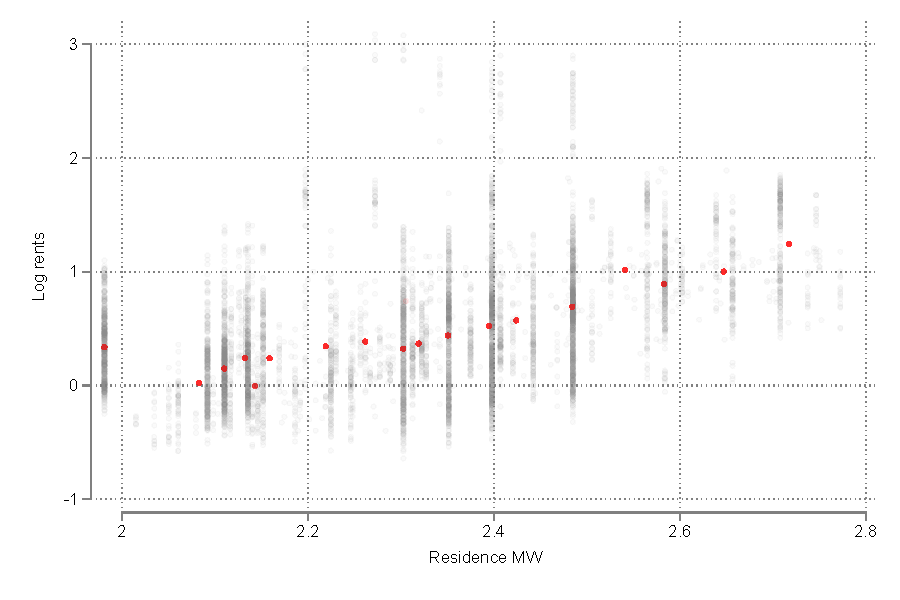
\includegraphics[width = 1\textwidth]{non_parametric/output/cbsa_month_mw_res.png}
    \end{subfigure}%
    \begin{subfigure}{0.45\textwidth}
        \caption{Residence MW, raw data}
        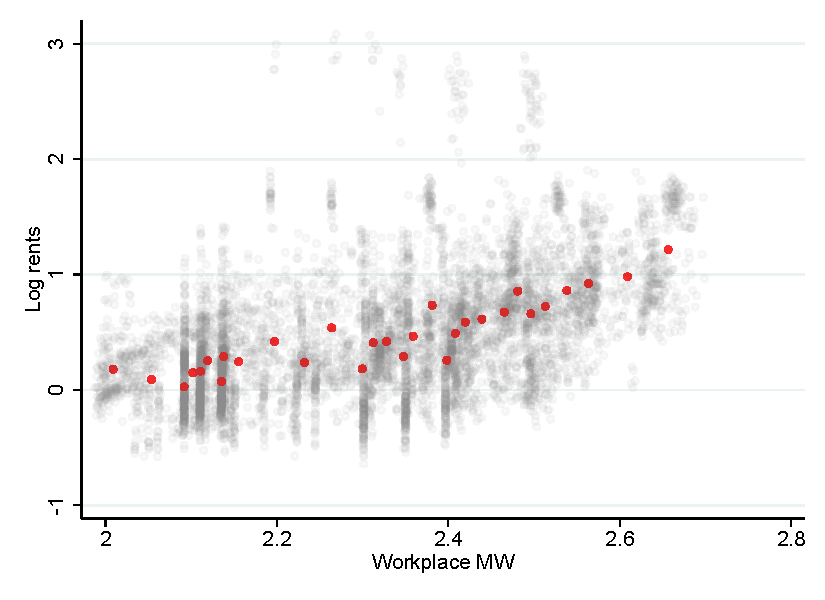
\includegraphics[width = 1\textwidth]{non_parametric/output/cbsa_month_mw_wkp.png}
    \end{subfigure}\\
    \begin{subfigure}{0.45\textwidth}
        \caption{Workplace MW, conditional on ZIP\\code and residence
        MW indicators}

        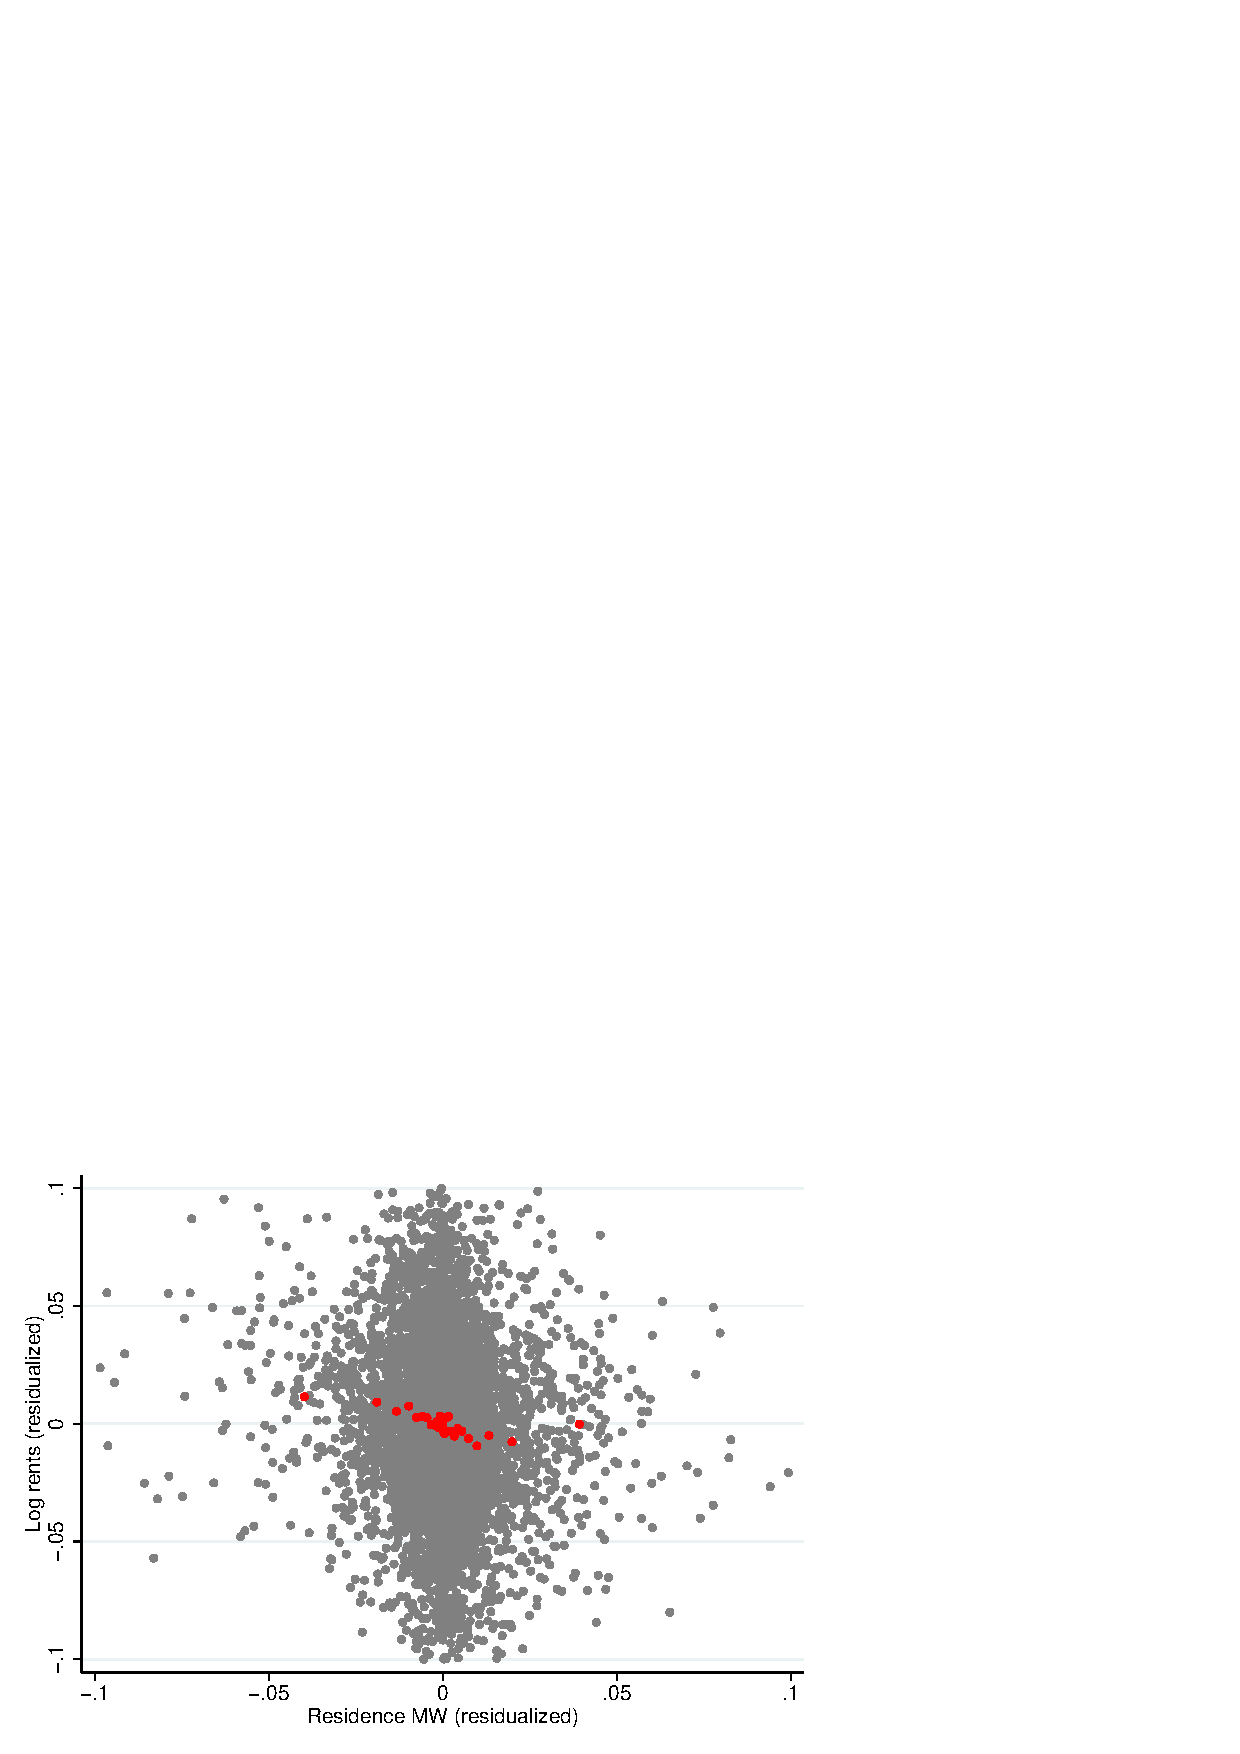
\includegraphics[width = 1\textwidth]{non_parametric/output/cbsa_month_mw_res_resid_mw_wkp_dec.png}
    \end{subfigure}%
    \begin{subfigure}{0.45\textwidth}
        \caption{Residence MW, conditional on ZIP\\code and workplace
        MW indicators}

        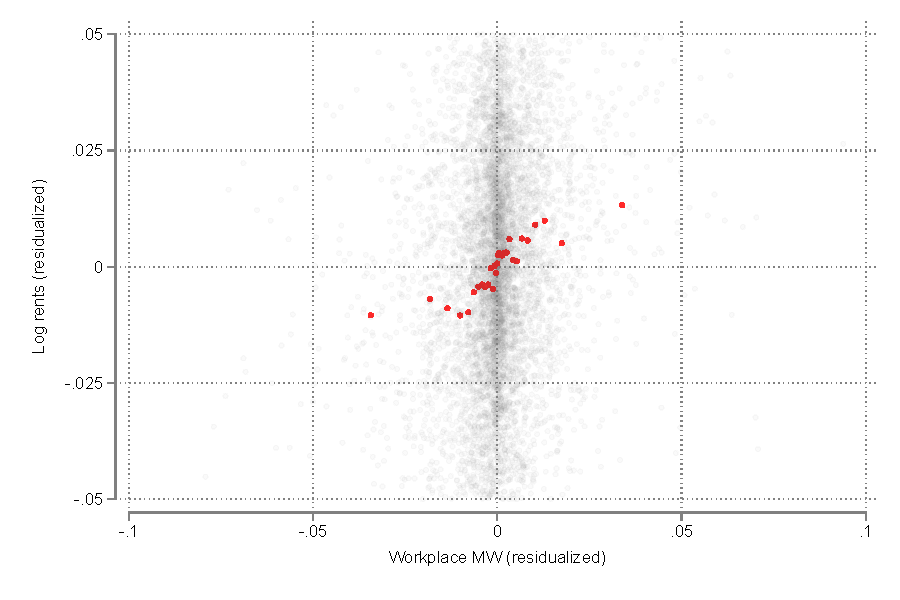
\includegraphics[width = 1\textwidth]{non_parametric/output/cbsa_month_mw_wkp_resid_mw_res_dec.png}
    \end{subfigure} 

    \begin{minipage}{.95\textwidth} \footnotesize
        \vspace{3mm}
        Notes:
        Data are from Zillow and LODES. We keep in the sample ZIP code-month
        observations located in CBSAs where there was some MW increase in the 
        month of interest. Rents correspond to log rents per square foot in
        SFCC category. The workplace MW measeure uses LODES data from the 
        closest prior year. The top row shows the raw relationship between log 
        rents and workplace and residence minimum wage. The bottom row
        shows the same relationship using residuals from regressions on ZIP 
        code and 100 residence/workplace MW indicators. Red dots are 30 
        equally-sized bins of the $x$-axis variable. 
    \end{minipage}
\end{figure}